% ============================
% TP Report – Simple Two-Column Template
% ============================
\documentclass[10pt,a4paper,twocolumn]{article}

% ---- Encoding & typography (simple, portable) ----
\usepackage[utf8]{inputenc}
\usepackage[T1]{fontenc}
\usepackage{lmodern}
\usepackage{microtype}

% ---- Layout ----
\usepackage{geometry}
\geometry{
  left=1.4cm, right=1.4cm,
  top=1.5cm, bottom=1.5cm,
  columnsep=0.55cm
}
\usepackage{balance} % balances the final page columns

% ---- Graphics ----
\usepackage{graphicx}
\usepackage[font=small,labelfont=bf]{caption}

% ---- Useful tweaks (optional) ----
\setlength{\parskip}{0pt}   % compact paragraphs
\setlength{\parindent}{1em} % classic indent; comment out if you prefer no indents

% ============================
%            Title
% ============================
\title{\vspace{-6mm}\textbf{TP1: Identification d’un Système Mécanique
Linéaire}}
\author{Léo Sabatié, Esteban Peregrina\quad (Groupe 2, ROB5) \\ Instructor: Mahdi Khoramshahi \quad School: Polytech Sorbonne}
\date{\today}

\begin{document}
\maketitle

% ============================
%         One-sentence intro
% ============================
% Keep this to 2–3 lines max; no abstract section to stay minimal.
\noindent\textbf{Context.} Ce premier TP d'identification paramétrique 
nous introduit aux concepts fondamentaux de cette UE en proposant d'étudier un système 
mécanique linéaire dont on connaît les paramètres. On y compare l'erreur sur chaque paramètre
selon les mesures utilisées et le traitement qu'on leur applique (quantification virtuelle, filtrage...).

% ============================
%           Sections
% ============================
\section*{Etude Théorique}
Le système mécanique étudié est constitué de trois masses et comporte
neuf paramètres à identifier :
les raideurs $k_0$, $k_1$, $k_2$, les coefficients d'amortissement
$b_0$, $b_1$, $b_2$ et les masses $m_1$, $m_2$, $m_3$.
Pour une mesure, les trois équations dynamiques fournissent trois
équations linéaires. Il faut donc au minimum trois mesures indépendantes
pour obtenir neuf équations et pouvoir identifier les neuf paramètres.

Le problème peut alors s'écrire sous la forme
\[
A p = Y,
\]
où $p$ est le vecteur des neuf paramètres recherchés.

\section*{Simulation du système}
Le système est simulé sous MATLAB à partir de ses fonctions de transfert.
Une force en échelon unitaire est appliquée et permet d'obtenir les
positions $\alpha$, $\beta$ et $\gamma$, ainsi que leurs vitesses et
accélérations.\\

% ============================
%     Main Results Figure
% ============================
% Use figure* to span both columns. Replace results.pdf with your image file.
\begin{figure}[!h]
  \centering
  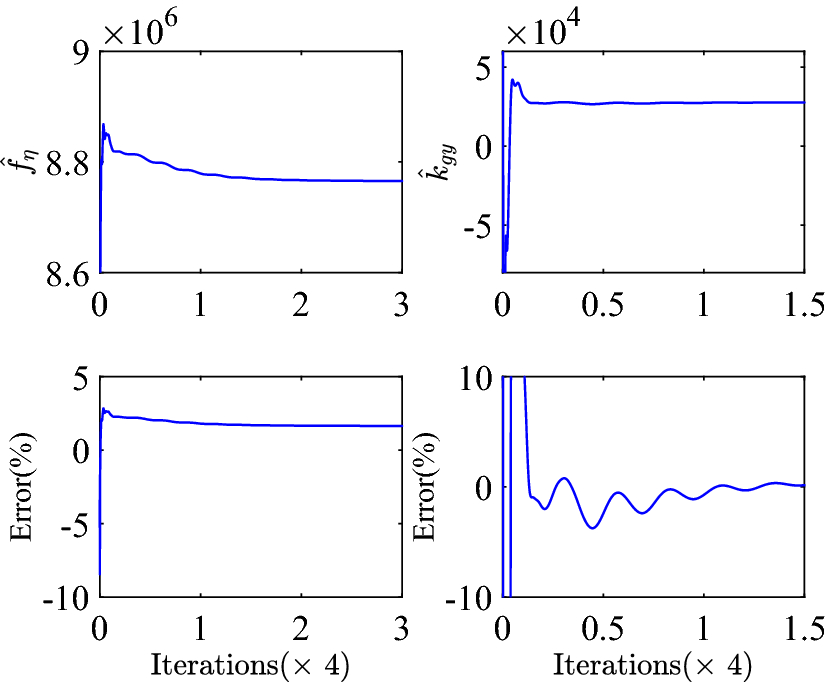
\includegraphics[width=0.30\textwidth]{fig_parameters.png}
  \caption{Réponse du système à un échelon unitaire de force.}
  \label{fig:summary}
\end{figure}

Les données obtenues constituent ensuite les mesures utilisées pour
construire la matrice d'identification $A$.

\section*{Identification des paramètres}
L'identification est réalisée en résolvant le système $Ap=Y$ sous MATLAB.
Le choix des mesures utilisées est important : si les mesures sont trop
similaires, les lignes de $A$ deviennent proches et le problème est mal
conditionné. Il est donc nécessaire de disposer de mesures suffisamment
informatives afin d'obtenir une identification fiable.

Le nombre de conditionnement de $A$, ainsi que son rang, permettent
notamment d'évaluer la qualité du problème d'identification.

% ============================
% Quantification et filtrage
% ============================
\section*{Quantification et filtrage}

Les positions, vitesses et accélérations simulées sont ensuite quantifiées
avec les résolutions imposées dans le TP. Cette opération introduit une
erreur sur les mesures, qui se répercute directement sur l'identification.

Un filtrage des données quantifiées est également étudié. Nous avons
constaté que le filtrage ne conduit pas nécessairement à une meilleure
identification : en supprimant certaines composantes du signal, il peut
également supprimer des informations utiles à l'estimation des paramètres.
Le choix du paramètre du filtre doit donc être réalisé en comparant les
erreurs d'identification.

% ============================
% Etude complémentaire
% ============================
\section*{Étude complémentaire}

Lorsque $k_1$ et $b_1$ deviennent très grands, les deux premières masses
sont fortement couplées. On obtient alors approximativement
\[
\alpha\simeq\beta,\qquad
\dot{\alpha}\simeq\dot{\beta},\qquad
\ddot{\alpha}\simeq\ddot{\beta}.
\]

Les paramètres $k_1$ et $b_1$ ne peuvent alors plus être correctement
identifiés. Le modèle est donc réduit afin de ne conserver que les
paramètres identifiables :
\[
p_r =
[k_0,\ k_2,\ b_0,\ b_2,\ m_1+m_2,\ m_3]^T.
\]

Pour ce modèle réduit, nous obtenons $\mathrm{cond}(A)=98$.
Les erreurs obtenues sont notamment de $0.12\%$ pour $k_0$,
$1.22\%$ pour $b_0$, $4.30\%$ pour $b_2$ et $4.84\%$ pour $m_3$.
L'erreur sur $m_1+m_2$ reste cependant plus importante, avec $33.35\%$.

% ============================
% Conclusion
% ============================
\section*{Conclusion}

Ce TP nous a permis de comprendre le principe de l'identification
paramétrique à partir de mesures simulées. Nous avons appris à construire
une matrice d'identification, à analyser son conditionnement et à étudier
l'influence de la quantification et du filtrage sur les résultats.

L'étude complémentaire montre également qu'un paramètre peut devenir
non identifiable lorsque les mesures ne contiennent plus suffisamment
d'information pour le distinguer. Il est alors nécessaire d'adapter le
modèle d'identification aux paramètres réellement observables.

\balance
\end{document}